\documentclass[11pt,a4paper,DIV20]{scrartcl}
\usepackage{amsmath}
\usepackage{amssymb}
\usepackage{graphicx}
\usepackage{multicol}
\usepackage[compat=1.1.0]{tikz-feynman}
\usetikzlibrary{shapes}

\title{Diagrams (total \# 28)\\[-0.5em]}
\author{\ttfamily{Richard\_Draw.py}}
\date{}

\begin{document}
\maketitle
\centering
\begin{verbatim}
----------------------------------------------------
 output = 'diagrams.dat' ;
 style = '../../richard_draw.sty' ;
 model = '../effective_counter.lag' ;
 in = fb[q1],fB[q2],effextQ[qc];
 out = fe[q3],fE[q4];
 loops = 1 ;
 loop_momentum = p ;
 options = onshell;
 true = iprop[effQ1,effQ2,0,2];
 false = iprop[effQ1,effQ2,1,1];
----------------------------------------------------
\end{verbatim}
\begin{minipage}[]{0.32\textwidth}
\begin{center}
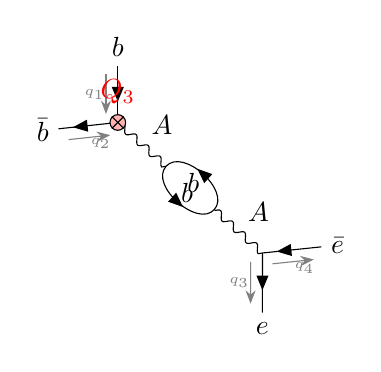
\begin{tikzpicture}
\tikzfeynmanset{}
\begin{feynman}
\diagram[small]{
   i1 [particle=$b$] -- [fermion, momentum'={[arrow style=gray, label distance=-1mm, arrow distance=1.5mm] {\tiny $q_{1}$}}] v4,
   i3 [particle=$\bar b$] -- [anti fermion, momentum'={[arrow style=gray, label distance=-1mm, arrow distance=1.5mm] {\tiny $q_{2}$}}] v4,
   v1 -- [fermion, momentum'={[arrow style=gray, label distance=-1mm, arrow distance=1.5mm] {\tiny $q_{3}$}}] o2 [particle=$e$], 
   v1 -- [anti fermion, momentum'={[arrow style=gray, label distance=-1mm, arrow distance=1.5mm] {\tiny $q_{4}$}}] o4 [particle=$\bar e$], 
   v2 -- [edge label=$A$, boson] v1,
   v3 -- [edge label=$b$, fermion, out=-90, in=-90, looseness = 1, relative=true] v2,
   v2 -- [edge label=$b$, fermion, out=-90, in=-90, looseness = 1, relative=true] v3,
   v4 -- [edge label=$A$, boson] v3,
};
\draw (v4) node [draw=black, shape=crossed circle, inner sep=2pt, fill=white!70!red, label={[red]$Q_3$}];
\end{feynman}
\end{tikzpicture}\\
\# $1$ \\
(symmetry: $-1$)
\end{center}
\end{minipage}
%
\begin{minipage}[]{0.32\textwidth}
\begin{center}
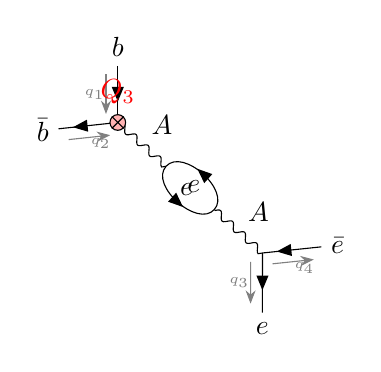
\begin{tikzpicture}
\tikzfeynmanset{}
\begin{feynman}
\diagram[small]{
   i1 [particle=$b$] -- [fermion, momentum'={[arrow style=gray, label distance=-1mm, arrow distance=1.5mm] {\tiny $q_{1}$}}] v4,
   i3 [particle=$\bar b$] -- [anti fermion, momentum'={[arrow style=gray, label distance=-1mm, arrow distance=1.5mm] {\tiny $q_{2}$}}] v4,
   v1 -- [fermion, momentum'={[arrow style=gray, label distance=-1mm, arrow distance=1.5mm] {\tiny $q_{3}$}}] o2 [particle=$e$], 
   v1 -- [anti fermion, momentum'={[arrow style=gray, label distance=-1mm, arrow distance=1.5mm] {\tiny $q_{4}$}}] o4 [particle=$\bar e$], 
   v2 -- [edge label=$A$, boson] v1,
   v3 -- [edge label=$e$, fermion, out=-90, in=-90, looseness = 1, relative=true] v2,
   v2 -- [edge label=$e$, fermion, out=-90, in=-90, looseness = 1, relative=true] v3,
   v4 -- [edge label=$A$, boson] v3,
};
\draw (v4) node [draw=black, shape=crossed circle, inner sep=2pt, fill=white!70!red, label={[red]$Q_3$}];
\end{feynman}
\end{tikzpicture}\\
\# $2$ \\
(symmetry: $-1$)
\end{center}
\end{minipage}
%
\begin{minipage}[]{0.32\textwidth}
\begin{center}
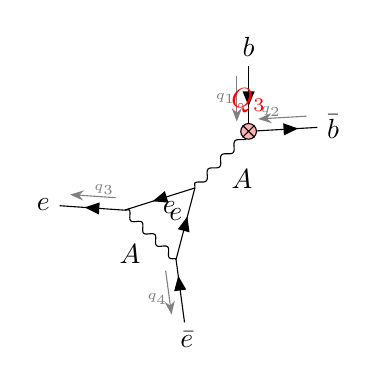
\begin{tikzpicture}
\tikzfeynmanset{}
\begin{feynman}
\diagram[small]{
   i1 [particle=$b$] -- [fermion, momentum'={[arrow style=gray, label distance=-1mm, arrow distance=1.5mm] {\tiny $q_{1}$}}] v4,
   i3 [particle=$\bar b$] -- [anti fermion, momentum'={[arrow style=gray, label distance=-1mm, arrow distance=1.5mm] {\tiny $q_{2}$}}] v4,
   v1 -- [fermion, momentum'={[arrow style=gray, label distance=-1mm, arrow distance=1.5mm] {\tiny $q_{3}$}}] o2 [particle=$e$], 
   v2 -- [anti fermion, momentum'={[arrow style=gray, label distance=-1mm, arrow distance=1.5mm] {\tiny $q_{4}$}}] o4 [particle=$\bar e$], 
   v2 -- [edge label=$A$, boson] v1,
   v3 -- [edge label=$e$, fermion] v1,
   v2 -- [edge label=$e$, fermion] v3,
   v4 -- [edge label=$A$, boson] v3,
};
\draw (v4) node [draw=black, shape=crossed circle, inner sep=2pt, fill=white!70!red, label={[red]$Q_3$}];
\end{feynman}
\end{tikzpicture}\\
\# $3$ \\
(symmetry: $+1$)
\end{center}
\end{minipage}
%
\begin{minipage}[]{0.32\textwidth}
\begin{center}
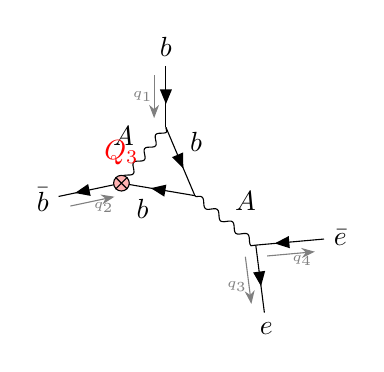
\begin{tikzpicture}
\tikzfeynmanset{}
\begin{feynman}
\diagram[small]{
   i1 [particle=$b$] -- [fermion, momentum'={[arrow style=gray, label distance=-1mm, arrow distance=1.5mm] {\tiny $q_{1}$}}] v2,
   i3 [particle=$\bar b$] -- [anti fermion, momentum'={[arrow style=gray, label distance=-1mm, arrow distance=1.5mm] {\tiny $q_{2}$}}] v4,
   v1 -- [fermion, momentum'={[arrow style=gray, label distance=-1mm, arrow distance=1.5mm] {\tiny $q_{3}$}}] o2 [particle=$e$], 
   v1 -- [anti fermion, momentum'={[arrow style=gray, label distance=-1mm, arrow distance=1.5mm] {\tiny $q_{4}$}}] o4 [particle=$\bar e$], 
   v3 -- [edge label=$A$, boson] v1,
   v2 -- [edge label=$b$, fermion] v3,
   v4 -- [edge label=$A$, boson] v2,
   v3 -- [edge label=$b$, fermion] v4,
};
\draw (v4) node [draw=black, shape=crossed circle, inner sep=2pt, fill=white!70!red, label={[red]$Q_3$}];
\end{feynman}
\end{tikzpicture}\\
\# $4$ \\
(symmetry: $+1$)
\end{center}
\end{minipage}
%
\begin{minipage}[]{0.32\textwidth}
\begin{center}
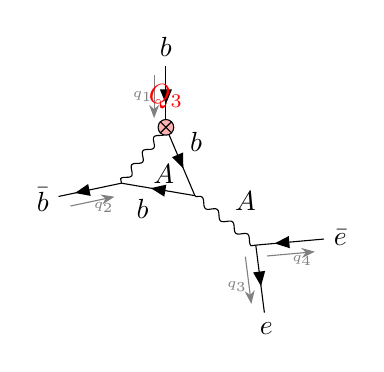
\begin{tikzpicture}
\tikzfeynmanset{}
\begin{feynman}
\diagram[small]{
   i1 [particle=$b$] -- [fermion, momentum'={[arrow style=gray, label distance=-1mm, arrow distance=1.5mm] {\tiny $q_{1}$}}] v4,
   i3 [particle=$\bar b$] -- [anti fermion, momentum'={[arrow style=gray, label distance=-1mm, arrow distance=1.5mm] {\tiny $q_{2}$}}] v2,
   v1 -- [fermion, momentum'={[arrow style=gray, label distance=-1mm, arrow distance=1.5mm] {\tiny $q_{3}$}}] o2 [particle=$e$], 
   v1 -- [anti fermion, momentum'={[arrow style=gray, label distance=-1mm, arrow distance=1.5mm] {\tiny $q_{4}$}}] o4 [particle=$\bar e$], 
   v3 -- [edge label=$A$, boson] v1,
   v3 -- [edge label=$b$, fermion] v2,
   v4 -- [edge label=$A$, boson] v2,
   v4 -- [edge label=$b$, fermion] v3,
};
\draw (v4) node [draw=black, shape=crossed circle, inner sep=2pt, fill=white!70!red, label={[red]$Q_3$}];
\end{feynman}
\end{tikzpicture}\\
\# $5$ \\
(symmetry: $+1$)
\end{center}
\end{minipage}
%
\begin{minipage}[]{0.32\textwidth}
\begin{center}
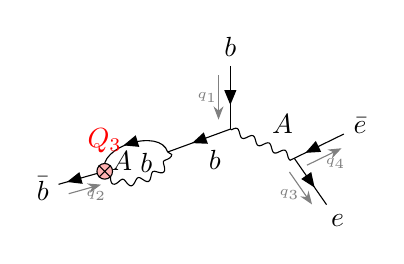
\begin{tikzpicture}
\tikzfeynmanset{}
\begin{feynman}
\diagram[small]{
   i1 [particle=$b$] -- [fermion, momentum'={[arrow style=gray, label distance=-1mm, arrow distance=1.5mm] {\tiny $q_{1}$}}] v2,
   i3 [particle=$\bar b$] -- [anti fermion, momentum'={[arrow style=gray, label distance=-1mm, arrow distance=1.5mm] {\tiny $q_{2}$}}] v4,
   v1 -- [fermion, momentum'={[arrow style=gray, label distance=-1mm, arrow distance=1.5mm] {\tiny $q_{3}$}}] o2 [particle=$e$], 
   v1 -- [anti fermion, momentum'={[arrow style=gray, label distance=-1mm, arrow distance=1.5mm] {\tiny $q_{4}$}}] o4 [particle=$\bar e$], 
   v2 -- [edge label=$A$, boson] v1,
   v2 -- [edge label=$b$, fermion] v3,
   v4 -- [edge label=$A$, boson, out=-90, in=-90, looseness = 1, relative=true] v3,
   v3 -- [edge label=$b$, fermion, out=-90, in=-90, looseness = 1, relative=true] v4,
};
\draw (v4) node [draw=black, shape=crossed circle, inner sep=2pt, fill=white!70!red, label={[red]$Q_3$}];
\end{feynman}
\end{tikzpicture}\\
\# $6$ \\
(symmetry: $+1$)
\end{center}
\end{minipage}
%
\begin{minipage}[]{0.32\textwidth}
\begin{center}
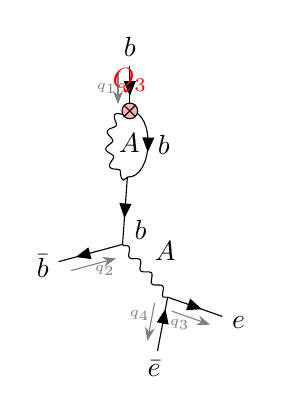
\begin{tikzpicture}
\tikzfeynmanset{}
\begin{feynman}
\diagram[small]{
   i1 [particle=$b$] -- [fermion, momentum'={[arrow style=gray, label distance=-1mm, arrow distance=1.5mm] {\tiny $q_{1}$}}] v4,
   i3 [particle=$\bar b$] -- [anti fermion, momentum'={[arrow style=gray, label distance=-1mm, arrow distance=1.5mm] {\tiny $q_{2}$}}] v2,
   v1 -- [fermion, momentum'={[arrow style=gray, label distance=-1mm, arrow distance=1.5mm] {\tiny $q_{3}$}}] o2 [particle=$e$], 
   v1 -- [anti fermion, momentum'={[arrow style=gray, label distance=-1mm, arrow distance=1.5mm] {\tiny $q_{4}$}}] o4 [particle=$\bar e$], 
   v2 -- [edge label=$A$, boson] v1,
   v3 -- [edge label=$b$, fermion] v2,
   v4 -- [edge label=$A$, boson, out=-90, in=-90, looseness = 1, relative=true] v3,
   v4 -- [edge label=$b$, fermion, out=90, in=90, looseness = 1, relative=true] v3,
};
\draw (v4) node [draw=black, shape=crossed circle, inner sep=2pt, fill=white!70!red, label={[red]$Q_3$}];
\end{feynman}
\end{tikzpicture}\\
\# $7$ \\
(symmetry: $+1$)
\end{center}
\end{minipage}
%
\begin{minipage}[]{0.32\textwidth}
\begin{center}
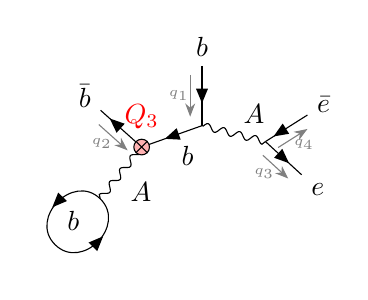
\begin{tikzpicture}
\tikzfeynmanset{}
\begin{feynman}
\diagram[small]{
   i1 [particle=$b$] -- [fermion, momentum'={[arrow style=gray, label distance=-1mm, arrow distance=1.5mm] {\tiny $q_{1}$}}] v2,
   i3 [particle=$\bar b$] -- [anti fermion, momentum'={[arrow style=gray, label distance=-1mm, arrow distance=1.5mm] {\tiny $q_{2}$}}] v4,
   v1 -- [fermion, momentum'={[arrow style=gray, label distance=-1mm, arrow distance=1.5mm] {\tiny $q_{3}$}}] o2 [particle=$e$], 
   v1 -- [anti fermion, momentum'={[arrow style=gray, label distance=-1mm, arrow distance=1.5mm] {\tiny $q_{4}$}}] o4 [particle=$\bar e$], 
   v3 -- [half right, edge label=$b$, fermion] t3,
   t3 -- [half right, fermion] v3,
   v2 -- [edge label=$A$, boson] v1,
   v2 -- [edge label=$b$, fermion] v4,
   v4 -- [edge label=$A$, boson] v3,
};
\draw (v4) node [draw=black, shape=crossed circle, inner sep=2pt, fill=white!70!red, label={[red]$Q_3$}];
\end{feynman}
\end{tikzpicture}\\
\# $8$ \\
(symmetry: $-1$)
\end{center}
\end{minipage}
%
\begin{minipage}[]{0.32\textwidth}
\begin{center}
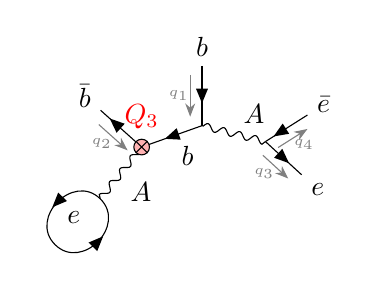
\begin{tikzpicture}
\tikzfeynmanset{}
\begin{feynman}
\diagram[small]{
   i1 [particle=$b$] -- [fermion, momentum'={[arrow style=gray, label distance=-1mm, arrow distance=1.5mm] {\tiny $q_{1}$}}] v2,
   i3 [particle=$\bar b$] -- [anti fermion, momentum'={[arrow style=gray, label distance=-1mm, arrow distance=1.5mm] {\tiny $q_{2}$}}] v4,
   v1 -- [fermion, momentum'={[arrow style=gray, label distance=-1mm, arrow distance=1.5mm] {\tiny $q_{3}$}}] o2 [particle=$e$], 
   v1 -- [anti fermion, momentum'={[arrow style=gray, label distance=-1mm, arrow distance=1.5mm] {\tiny $q_{4}$}}] o4 [particle=$\bar e$], 
   v3 -- [half right, edge label=$e$, fermion] t3,
   t3 -- [half right, fermion] v3,
   v2 -- [edge label=$A$, boson] v1,
   v2 -- [edge label=$b$, fermion] v4,
   v4 -- [edge label=$A$, boson] v3,
};
\draw (v4) node [draw=black, shape=crossed circle, inner sep=2pt, fill=white!70!red, label={[red]$Q_3$}];
\end{feynman}
\end{tikzpicture}\\
\# $9$ \\
(symmetry: $-1$)
\end{center}
\end{minipage}
%
\begin{minipage}[]{0.32\textwidth}
\begin{center}
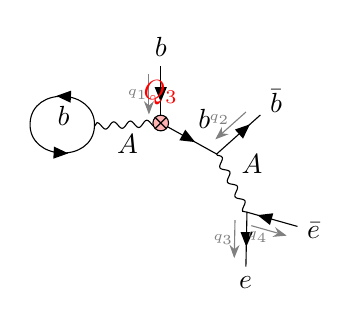
\begin{tikzpicture}
\tikzfeynmanset{}
\begin{feynman}
\diagram[small]{
   i1 [particle=$b$] -- [fermion, momentum'={[arrow style=gray, label distance=-1mm, arrow distance=1.5mm] {\tiny $q_{1}$}}] v4,
   i3 [particle=$\bar b$] -- [anti fermion, momentum'={[arrow style=gray, label distance=-1mm, arrow distance=1.5mm] {\tiny $q_{2}$}}] v2,
   v1 -- [fermion, momentum'={[arrow style=gray, label distance=-1mm, arrow distance=1.5mm] {\tiny $q_{3}$}}] o2 [particle=$e$], 
   v1 -- [anti fermion, momentum'={[arrow style=gray, label distance=-1mm, arrow distance=1.5mm] {\tiny $q_{4}$}}] o4 [particle=$\bar e$], 
   v3 -- [half right, edge label=$b$, fermion] t3,
   t3 -- [half right, fermion] v3,
   v2 -- [edge label=$A$, boson] v1,
   v4 -- [edge label=$b$, fermion] v2,
   v4 -- [edge label=$A$, boson] v3,
};
\draw (v4) node [draw=black, shape=crossed circle, inner sep=2pt, fill=white!70!red, label={[red]$Q_3$}];
\end{feynman}
\end{tikzpicture}\\
\# $10$ \\
(symmetry: $-1$)
\end{center}
\end{minipage}
%
\begin{minipage}[]{0.32\textwidth}
\begin{center}
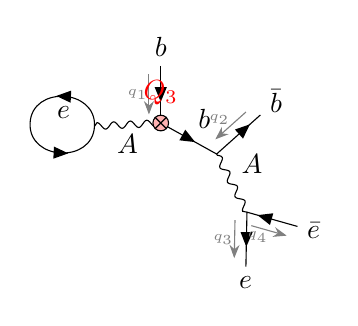
\begin{tikzpicture}
\tikzfeynmanset{}
\begin{feynman}
\diagram[small]{
   i1 [particle=$b$] -- [fermion, momentum'={[arrow style=gray, label distance=-1mm, arrow distance=1.5mm] {\tiny $q_{1}$}}] v4,
   i3 [particle=$\bar b$] -- [anti fermion, momentum'={[arrow style=gray, label distance=-1mm, arrow distance=1.5mm] {\tiny $q_{2}$}}] v2,
   v1 -- [fermion, momentum'={[arrow style=gray, label distance=-1mm, arrow distance=1.5mm] {\tiny $q_{3}$}}] o2 [particle=$e$], 
   v1 -- [anti fermion, momentum'={[arrow style=gray, label distance=-1mm, arrow distance=1.5mm] {\tiny $q_{4}$}}] o4 [particle=$\bar e$], 
   v3 -- [half right, edge label=$e$, fermion] t3,
   t3 -- [half right, fermion] v3,
   v2 -- [edge label=$A$, boson] v1,
   v4 -- [edge label=$b$, fermion] v2,
   v4 -- [edge label=$A$, boson] v3,
};
\draw (v4) node [draw=black, shape=crossed circle, inner sep=2pt, fill=white!70!red, label={[red]$Q_3$}];
\end{feynman}
\end{tikzpicture}\\
\# $11$ \\
(symmetry: $-1$)
\end{center}
\end{minipage}
%
\begin{minipage}[]{0.32\textwidth}
\begin{center}
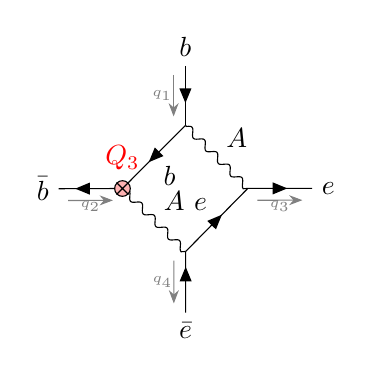
\begin{tikzpicture}
\tikzfeynmanset{}
\begin{feynman}
\diagram[small]{
   i1 [particle=$b$] -- [fermion, momentum'={[arrow style=gray, label distance=-1mm, arrow distance=1.5mm] {\tiny $q_{1}$}}] v2,
   i3 [particle=$\bar b$] -- [anti fermion, momentum'={[arrow style=gray, label distance=-1mm, arrow distance=1.5mm] {\tiny $q_{2}$}}] v4,
   v1 -- [fermion, momentum'={[arrow style=gray, label distance=-1mm, arrow distance=1.5mm] {\tiny $q_{3}$}}] o2 [particle=$e$], 
   v3 -- [anti fermion, momentum'={[arrow style=gray, label distance=-1mm, arrow distance=1.5mm] {\tiny $q_{4}$}}] o4 [particle=$\bar e$], 
   v2 -- [edge label=$A$, boson] v1,
   v3 -- [edge label=$e$, fermion] v1,
   v2 -- [edge label=$b$, fermion] v4,
   v4 -- [edge label=$A$, boson] v3,
};
\draw (v4) node [draw=black, shape=crossed circle, inner sep=2pt, fill=white!70!red, label={[red]$Q_3$}];
\end{feynman}
\end{tikzpicture}\\
\# $12$ \\
(symmetry: $+1$)
\end{center}
\end{minipage}
%
\begin{minipage}[]{0.32\textwidth}
\begin{center}
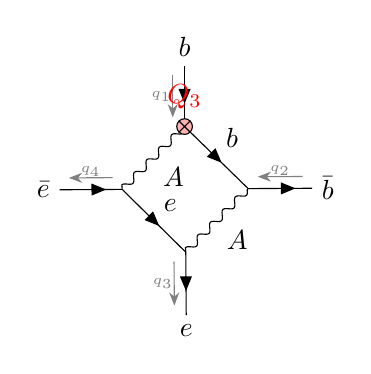
\begin{tikzpicture}
\tikzfeynmanset{}
\begin{feynman}
\diagram[small]{
   i1 [particle=$b$] -- [fermion, momentum'={[arrow style=gray, label distance=-1mm, arrow distance=1.5mm] {\tiny $q_{1}$}}] v4,
   i3 [particle=$\bar b$] -- [anti fermion, momentum'={[arrow style=gray, label distance=-1mm, arrow distance=1.5mm] {\tiny $q_{2}$}}] v2,
   v1 -- [fermion, momentum'={[arrow style=gray, label distance=-1mm, arrow distance=1.5mm] {\tiny $q_{3}$}}] o2 [particle=$e$], 
   v3 -- [anti fermion, momentum'={[arrow style=gray, label distance=-1mm, arrow distance=1.5mm] {\tiny $q_{4}$}}] o4 [particle=$\bar e$], 
   v2 -- [edge label=$A$, boson] v1,
   v3 -- [edge label=$e$, fermion] v1,
   v4 -- [edge label=$b$, fermion] v2,
   v4 -- [edge label=$A$, boson] v3,
};
\draw (v4) node [draw=black, shape=crossed circle, inner sep=2pt, fill=white!70!red, label={[red]$Q_3$}];
\end{feynman}
\end{tikzpicture}\\
\# $13$ \\
(symmetry: $+1$)
\end{center}
\end{minipage}
%
\begin{minipage}[]{0.32\textwidth}
\begin{center}
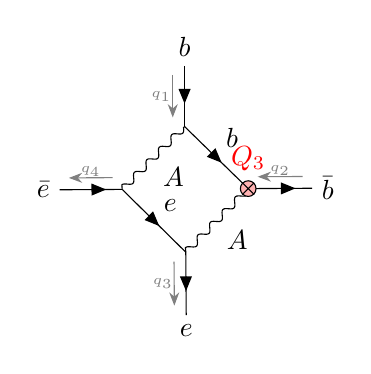
\begin{tikzpicture}
\tikzfeynmanset{}
\begin{feynman}
\diagram[small]{
   i1 [particle=$b$] -- [fermion, momentum'={[arrow style=gray, label distance=-1mm, arrow distance=1.5mm] {\tiny $q_{1}$}}] v2,
   i3 [particle=$\bar b$] -- [anti fermion, momentum'={[arrow style=gray, label distance=-1mm, arrow distance=1.5mm] {\tiny $q_{2}$}}] v4,
   v3 -- [fermion, momentum'={[arrow style=gray, label distance=-1mm, arrow distance=1.5mm] {\tiny $q_{3}$}}] o2 [particle=$e$], 
   v1 -- [anti fermion, momentum'={[arrow style=gray, label distance=-1mm, arrow distance=1.5mm] {\tiny $q_{4}$}}] o4 [particle=$\bar e$], 
   v2 -- [edge label=$A$, boson] v1,
   v1 -- [edge label=$e$, fermion] v3,
   v2 -- [edge label=$b$, fermion] v4,
   v4 -- [edge label=$A$, boson] v3,
};
\draw (v4) node [draw=black, shape=crossed circle, inner sep=2pt, fill=white!70!red, label={[red]$Q_3$}];
\end{feynman}
\end{tikzpicture}\\
\# $14$ \\
(symmetry: $+1$)
\end{center}
\end{minipage}
%
\begin{minipage}[]{0.32\textwidth}
\begin{center}
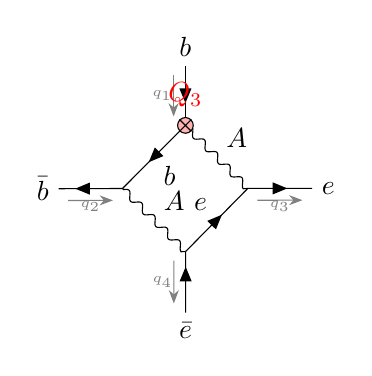
\begin{tikzpicture}
\tikzfeynmanset{}
\begin{feynman}
\diagram[small]{
   i1 [particle=$b$] -- [fermion, momentum'={[arrow style=gray, label distance=-1mm, arrow distance=1.5mm] {\tiny $q_{1}$}}] v4,
   i3 [particle=$\bar b$] -- [anti fermion, momentum'={[arrow style=gray, label distance=-1mm, arrow distance=1.5mm] {\tiny $q_{2}$}}] v2,
   v3 -- [fermion, momentum'={[arrow style=gray, label distance=-1mm, arrow distance=1.5mm] {\tiny $q_{3}$}}] o2 [particle=$e$], 
   v1 -- [anti fermion, momentum'={[arrow style=gray, label distance=-1mm, arrow distance=1.5mm] {\tiny $q_{4}$}}] o4 [particle=$\bar e$], 
   v2 -- [edge label=$A$, boson] v1,
   v1 -- [edge label=$e$, fermion] v3,
   v4 -- [edge label=$b$, fermion] v2,
   v4 -- [edge label=$A$, boson] v3,
};
\draw (v4) node [draw=black, shape=crossed circle, inner sep=2pt, fill=white!70!red, label={[red]$Q_3$}];
\end{feynman}
\end{tikzpicture}\\
\# $15$ \\
(symmetry: $+1$)
\end{center}
\end{minipage}
%
\begin{minipage}[]{0.32\textwidth}
\begin{center}
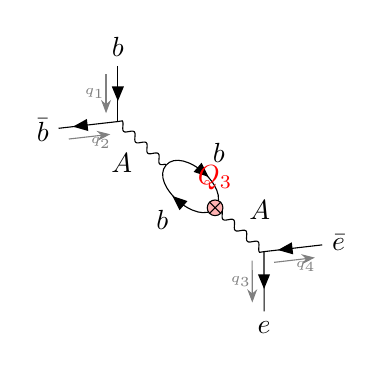
\begin{tikzpicture}
\tikzfeynmanset{}
\begin{feynman}
\diagram[small]{
   i1 [particle=$b$] -- [fermion, momentum'={[arrow style=gray, label distance=-1mm, arrow distance=1.5mm] {\tiny $q_{1}$}}] v1,
   i3 [particle=$\bar b$] -- [anti fermion, momentum'={[arrow style=gray, label distance=-1mm, arrow distance=1.5mm] {\tiny $q_{2}$}}] v1,
   v2 -- [fermion, momentum'={[arrow style=gray, label distance=-1mm, arrow distance=1.5mm] {\tiny $q_{3}$}}] o2 [particle=$e$], 
   v2 -- [anti fermion, momentum'={[arrow style=gray, label distance=-1mm, arrow distance=1.5mm] {\tiny $q_{4}$}}] o4 [particle=$\bar e$], 
   v3 -- [edge label=$A$, boson] v1,
   v4 -- [edge label=$A$, boson] v2,
   v3 -- [edge label=$b$, fermion, out=90, in=90, looseness = 1, relative=true] v4,
   v4 -- [edge label=$b$, fermion, out=90, in=90, looseness = 1, relative=true] v3,
};
\draw (v4) node [draw=black, shape=crossed circle, inner sep=2pt, fill=white!70!red, label={[red]$Q_3$}];
\end{feynman}
\end{tikzpicture}\\
\# $16$ \\
(symmetry: $-1$)
\end{center}
\end{minipage}
%
\begin{minipage}[]{0.32\textwidth}
\begin{center}
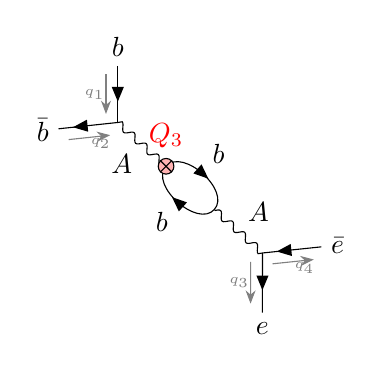
\begin{tikzpicture}
\tikzfeynmanset{}
\begin{feynman}
\diagram[small]{
   i1 [particle=$b$] -- [fermion, momentum'={[arrow style=gray, label distance=-1mm, arrow distance=1.5mm] {\tiny $q_{1}$}}] v2,
   i3 [particle=$\bar b$] -- [anti fermion, momentum'={[arrow style=gray, label distance=-1mm, arrow distance=1.5mm] {\tiny $q_{2}$}}] v2,
   v1 -- [fermion, momentum'={[arrow style=gray, label distance=-1mm, arrow distance=1.5mm] {\tiny $q_{3}$}}] o2 [particle=$e$], 
   v1 -- [anti fermion, momentum'={[arrow style=gray, label distance=-1mm, arrow distance=1.5mm] {\tiny $q_{4}$}}] o4 [particle=$\bar e$], 
   v3 -- [edge label=$A$, boson] v1,
   v4 -- [edge label=$A$, boson] v2,
   v3 -- [edge label=$b$, fermion, out=90, in=90, looseness = 1, relative=true] v4,
   v4 -- [edge label=$b$, fermion, out=90, in=90, looseness = 1, relative=true] v3,
};
\draw (v4) node [draw=black, shape=crossed circle, inner sep=2pt, fill=white!70!red, label={[red]$Q_3$}];
\end{feynman}
\end{tikzpicture}\\
\# $17$ \\
(symmetry: $-1$)
\end{center}
\end{minipage}
%
\begin{minipage}[]{0.32\textwidth}
\begin{center}
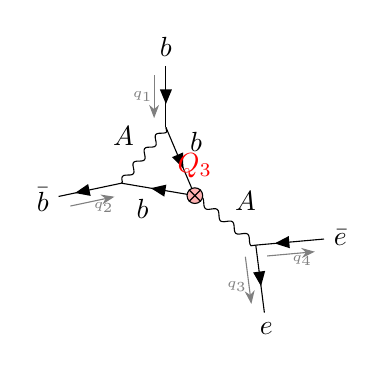
\begin{tikzpicture}
\tikzfeynmanset{}
\begin{feynman}
\diagram[small]{
   i1 [particle=$b$] -- [fermion, momentum'={[arrow style=gray, label distance=-1mm, arrow distance=1.5mm] {\tiny $q_{1}$}}] v2,
   i3 [particle=$\bar b$] -- [anti fermion, momentum'={[arrow style=gray, label distance=-1mm, arrow distance=1.5mm] {\tiny $q_{2}$}}] v3,
   v1 -- [fermion, momentum'={[arrow style=gray, label distance=-1mm, arrow distance=1.5mm] {\tiny $q_{3}$}}] o2 [particle=$e$], 
   v1 -- [anti fermion, momentum'={[arrow style=gray, label distance=-1mm, arrow distance=1.5mm] {\tiny $q_{4}$}}] o4 [particle=$\bar e$], 
   v4 -- [edge label=$A$, boson] v1,
   v3 -- [edge label=$A$, boson] v2,
   v2 -- [edge label=$b$, fermion] v4,
   v4 -- [edge label=$b$, fermion] v3,
};
\draw (v4) node [draw=black, shape=crossed circle, inner sep=2pt, fill=white!70!red, label={[red]$Q_3$}];
\end{feynman}
\end{tikzpicture}\\
\# $18$ \\
(symmetry: $+1$)
\end{center}
\end{minipage}
%
\begin{minipage}[]{0.32\textwidth}
\begin{center}
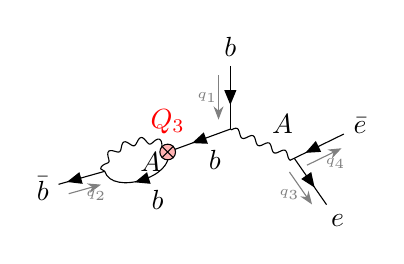
\begin{tikzpicture}
\tikzfeynmanset{}
\begin{feynman}
\diagram[small]{
   i1 [particle=$b$] -- [fermion, momentum'={[arrow style=gray, label distance=-1mm, arrow distance=1.5mm] {\tiny $q_{1}$}}] v2,
   i3 [particle=$\bar b$] -- [anti fermion, momentum'={[arrow style=gray, label distance=-1mm, arrow distance=1.5mm] {\tiny $q_{2}$}}] v3,
   v1 -- [fermion, momentum'={[arrow style=gray, label distance=-1mm, arrow distance=1.5mm] {\tiny $q_{3}$}}] o2 [particle=$e$], 
   v1 -- [anti fermion, momentum'={[arrow style=gray, label distance=-1mm, arrow distance=1.5mm] {\tiny $q_{4}$}}] o4 [particle=$\bar e$], 
   v2 -- [edge label=$A$, boson] v1,
   v2 -- [edge label=$b$, fermion] v4,
   v4 -- [edge label=$A$, boson, out=-90, in=-90, looseness = 1, relative=true] v3,
   v4 -- [edge label=$b$, fermion, out=90, in=90, looseness = 1, relative=true] v3,
};
\draw (v4) node [draw=black, shape=crossed circle, inner sep=2pt, fill=white!70!red, label={[red]$Q_3$}];
\end{feynman}
\end{tikzpicture}\\
\# $19$ \\
(symmetry: $+1$)
\end{center}
\end{minipage}
%
\begin{minipage}[]{0.32\textwidth}
\begin{center}
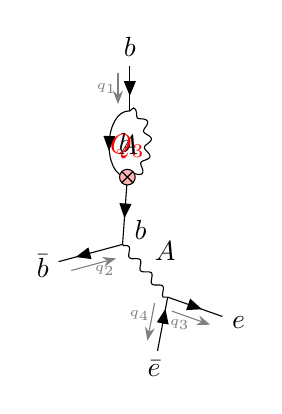
\begin{tikzpicture}
\tikzfeynmanset{}
\begin{feynman}
\diagram[small]{
   i1 [particle=$b$] -- [fermion, momentum'={[arrow style=gray, label distance=-1mm, arrow distance=1.5mm] {\tiny $q_{1}$}}] v3,
   i3 [particle=$\bar b$] -- [anti fermion, momentum'={[arrow style=gray, label distance=-1mm, arrow distance=1.5mm] {\tiny $q_{2}$}}] v2,
   v1 -- [fermion, momentum'={[arrow style=gray, label distance=-1mm, arrow distance=1.5mm] {\tiny $q_{3}$}}] o2 [particle=$e$], 
   v1 -- [anti fermion, momentum'={[arrow style=gray, label distance=-1mm, arrow distance=1.5mm] {\tiny $q_{4}$}}] o4 [particle=$\bar e$], 
   v2 -- [edge label=$A$, boson] v1,
   v4 -- [edge label=$b$, fermion] v2,
   v4 -- [edge label=$A$, boson, out=-90, in=-90, looseness = 1, relative=true] v3,
   v3 -- [edge label=$b$, fermion, out=-90, in=-90, looseness = 1, relative=true] v4,
};
\draw (v4) node [draw=black, shape=crossed circle, inner sep=2pt, fill=white!70!red, label={[red]$Q_3$}];
\end{feynman}
\end{tikzpicture}\\
\# $20$ \\
(symmetry: $+1$)
\end{center}
\end{minipage}
%
\begin{minipage}[]{0.32\textwidth}
\begin{center}
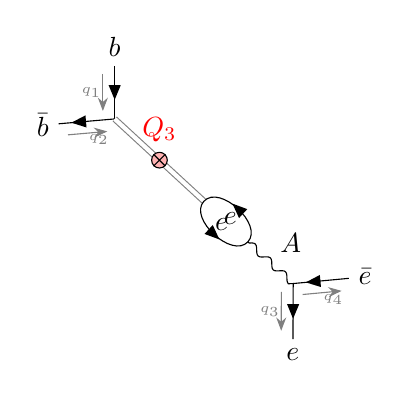
\begin{tikzpicture}
\tikzfeynmanset{}
\begin{feynman}
\diagram[small]{
   i1 [particle=$b$] -- [fermion, momentum'={[arrow style=gray, label distance=-1mm, arrow distance=1.5mm] {\tiny $q_{1}$}}] v1,
   i3 [particle=$\bar b$] -- [anti fermion, momentum'={[arrow style=gray, label distance=-1mm, arrow distance=1.5mm] {\tiny $q_{2}$}}] v1,
   v2 -- [fermion, momentum'={[arrow style=gray, label distance=-1mm, arrow distance=1.5mm] {\tiny $q_{3}$}}] o2 [particle=$e$], 
   v2 -- [anti fermion, momentum'={[arrow style=gray, label distance=-1mm, arrow distance=1.5mm] {\tiny $q_{4}$}}] o4 [particle=$\bar e$], 
   v3 -- [double distance=1.5pt, gray] v1,
   v4 -- [edge label=$A$, boson] v2,
   v5 -- [double distance=1.5pt, gray] v3,
   v5 -- [edge label=$e$, fermion, out=-90, in=-90, looseness = 1, relative=true] v4,
   v4 -- [edge label=$e$, fermion, out=-90, in=-90, looseness = 1, relative=true] v5,
};
\draw (v3) node [draw=black, shape=crossed circle, inner sep=2pt, fill=white!70!red, label={[red]$Q_3$}];
\end{feynman}
\end{tikzpicture}\\
\# $21$ \\
(symmetry: $-1$)
\end{center}
\end{minipage}
%
\begin{minipage}[]{0.32\textwidth}
\begin{center}
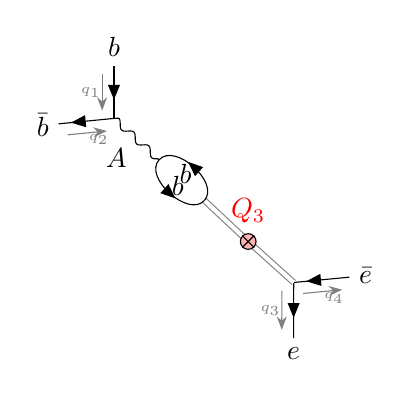
\begin{tikzpicture}
\tikzfeynmanset{}
\begin{feynman}
\diagram[small]{
   i1 [particle=$b$] -- [fermion, momentum'={[arrow style=gray, label distance=-1mm, arrow distance=1.5mm] {\tiny $q_{1}$}}] v2,
   i3 [particle=$\bar b$] -- [anti fermion, momentum'={[arrow style=gray, label distance=-1mm, arrow distance=1.5mm] {\tiny $q_{2}$}}] v2,
   v1 -- [fermion, momentum'={[arrow style=gray, label distance=-1mm, arrow distance=1.5mm] {\tiny $q_{3}$}}] o2 [particle=$e$], 
   v1 -- [anti fermion, momentum'={[arrow style=gray, label distance=-1mm, arrow distance=1.5mm] {\tiny $q_{4}$}}] o4 [particle=$\bar e$], 
   v3 -- [double distance=1.5pt, gray] v1,
   v4 -- [edge label=$A$, boson] v2,
   v5 -- [double distance=1.5pt, gray] v3,
   v5 -- [edge label=$b$, fermion, out=-90, in=-90, looseness = 1, relative=true] v4,
   v4 -- [edge label=$b$, fermion, out=-90, in=-90, looseness = 1, relative=true] v5,
};
\draw (v3) node [draw=black, shape=crossed circle, inner sep=2pt, fill=white!70!red, label={[red]$Q_3$}];
\end{feynman}
\end{tikzpicture}\\
\# $22$ \\
(symmetry: $-1$)
\end{center}
\end{minipage}
%
\begin{minipage}[]{0.32\textwidth}
\begin{center}
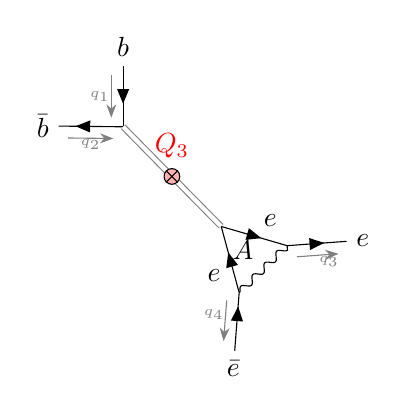
\begin{tikzpicture}
\tikzfeynmanset{}
\begin{feynman}
\diagram[small]{
   i1 [particle=$b$] -- [fermion, momentum'={[arrow style=gray, label distance=-1mm, arrow distance=1.5mm] {\tiny $q_{1}$}}] v1,
   i3 [particle=$\bar b$] -- [anti fermion, momentum'={[arrow style=gray, label distance=-1mm, arrow distance=1.5mm] {\tiny $q_{2}$}}] v1,
   v3 -- [fermion, momentum'={[arrow style=gray, label distance=-1mm, arrow distance=1.5mm] {\tiny $q_{3}$}}] o2 [particle=$e$], 
   v4 -- [anti fermion, momentum'={[arrow style=gray, label distance=-1mm, arrow distance=1.5mm] {\tiny $q_{4}$}}] o4 [particle=$\bar e$], 
   v2 -- [double distance=1.5pt, gray] v1,
   v5 -- [double distance=1.5pt, gray] v2,
   v4 -- [edge label=$A$, boson] v3,
   v5 -- [edge label=$e$, fermion] v3,
   v4 -- [edge label=$e$, fermion] v5,
};
\draw (v2) node [draw=black, shape=crossed circle, inner sep=2pt, fill=white!70!red, label={[red]$Q_3$}];
\end{feynman}
\end{tikzpicture}\\
\# $23$ \\
(symmetry: $+1$)
\end{center}
\end{minipage}
%
\begin{minipage}[]{0.32\textwidth}
\begin{center}
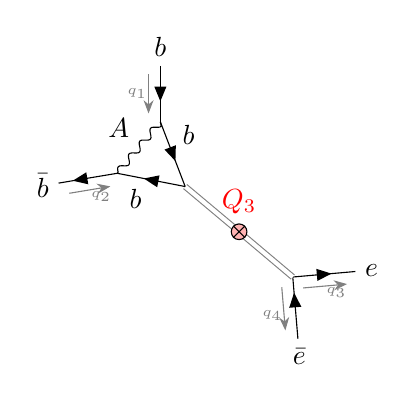
\begin{tikzpicture}
\tikzfeynmanset{}
\begin{feynman}
\diagram[small]{
   i1 [particle=$b$] -- [fermion, momentum'={[arrow style=gray, label distance=-1mm, arrow distance=1.5mm] {\tiny $q_{1}$}}] v3,
   i3 [particle=$\bar b$] -- [anti fermion, momentum'={[arrow style=gray, label distance=-1mm, arrow distance=1.5mm] {\tiny $q_{2}$}}] v4,
   v1 -- [fermion, momentum'={[arrow style=gray, label distance=-1mm, arrow distance=1.5mm] {\tiny $q_{3}$}}] o2 [particle=$e$], 
   v1 -- [anti fermion, momentum'={[arrow style=gray, label distance=-1mm, arrow distance=1.5mm] {\tiny $q_{4}$}}] o4 [particle=$\bar e$], 
   v2 -- [double distance=1.5pt, gray] v1,
   v5 -- [double distance=1.5pt, gray] v2,
   v4 -- [edge label=$A$, boson] v3,
   v3 -- [edge label=$b$, fermion] v5,
   v5 -- [edge label=$b$, fermion] v4,
};
\draw (v2) node [draw=black, shape=crossed circle, inner sep=2pt, fill=white!70!red, label={[red]$Q_3$}];
\end{feynman}
\end{tikzpicture}\\
\# $24$ \\
(symmetry: $+1$)
\end{center}
\end{minipage}
%
\begin{minipage}[]{0.32\textwidth}
\begin{center}
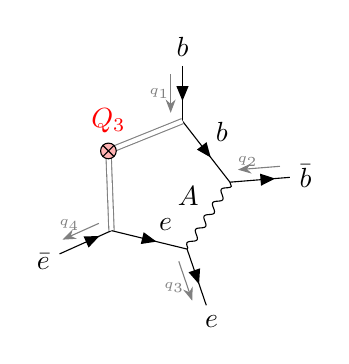
\begin{tikzpicture}
\tikzfeynmanset{}
\begin{feynman}
\diagram[small]{
   i1 [particle=$b$] -- [fermion, momentum'={[arrow style=gray, label distance=-1mm, arrow distance=1.5mm] {\tiny $q_{1}$}}] v1,
   i3 [particle=$\bar b$] -- [anti fermion, momentum'={[arrow style=gray, label distance=-1mm, arrow distance=1.5mm] {\tiny $q_{2}$}}] v2,
   v4 -- [fermion, momentum'={[arrow style=gray, label distance=-1mm, arrow distance=1.5mm] {\tiny $q_{3}$}}] o2 [particle=$e$], 
   v5 -- [anti fermion, momentum'={[arrow style=gray, label distance=-1mm, arrow distance=1.5mm] {\tiny $q_{4}$}}] o4 [particle=$\bar e$], 
   v1 -- [edge label=$b$, fermion] v2,
   v3 -- [double distance=1.5pt, gray] v1,
   v4 -- [edge label=$A$, boson] v2,
   v5 -- [double distance=1.5pt, gray] v3,
   v5 -- [edge label=$e$, fermion] v4,
};
\draw (v3) node [draw=black, shape=crossed circle, inner sep=2pt, fill=white!70!red, label={[red]$Q_3$}];
\end{feynman}
\end{tikzpicture}\\
\# $25$ \\
(symmetry: $+1$)
\end{center}
\end{minipage}
%
\begin{minipage}[]{0.32\textwidth}
\begin{center}
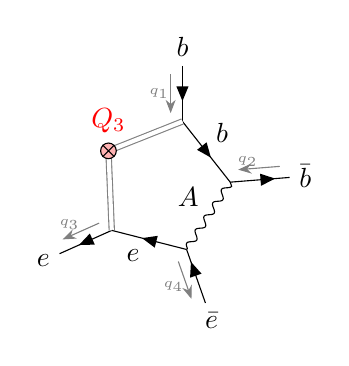
\begin{tikzpicture}
\tikzfeynmanset{}
\begin{feynman}
\diagram[small]{
   i1 [particle=$b$] -- [fermion, momentum'={[arrow style=gray, label distance=-1mm, arrow distance=1.5mm] {\tiny $q_{1}$}}] v1,
   i3 [particle=$\bar b$] -- [anti fermion, momentum'={[arrow style=gray, label distance=-1mm, arrow distance=1.5mm] {\tiny $q_{2}$}}] v2,
   v5 -- [fermion, momentum'={[arrow style=gray, label distance=-1mm, arrow distance=1.5mm] {\tiny $q_{3}$}}] o2 [particle=$e$], 
   v4 -- [anti fermion, momentum'={[arrow style=gray, label distance=-1mm, arrow distance=1.5mm] {\tiny $q_{4}$}}] o4 [particle=$\bar e$], 
   v1 -- [edge label=$b$, fermion] v2,
   v3 -- [double distance=1.5pt, gray] v1,
   v4 -- [edge label=$A$, boson] v2,
   v5 -- [double distance=1.5pt, gray] v3,
   v4 -- [edge label=$e$, fermion] v5,
};
\draw (v3) node [draw=black, shape=crossed circle, inner sep=2pt, fill=white!70!red, label={[red]$Q_3$}];
\end{feynman}
\end{tikzpicture}\\
\# $26$ \\
(symmetry: $+1$)
\end{center}
\end{minipage}
%
\begin{minipage}[]{0.32\textwidth}
\begin{center}
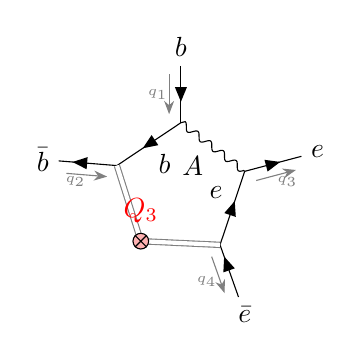
\begin{tikzpicture}
\tikzfeynmanset{}
\begin{feynman}
\diagram[small]{
   i1 [particle=$b$] -- [fermion, momentum'={[arrow style=gray, label distance=-1mm, arrow distance=1.5mm] {\tiny $q_{1}$}}] v1,
   i3 [particle=$\bar b$] -- [anti fermion, momentum'={[arrow style=gray, label distance=-1mm, arrow distance=1.5mm] {\tiny $q_{2}$}}] v2,
   v3 -- [fermion, momentum'={[arrow style=gray, label distance=-1mm, arrow distance=1.5mm] {\tiny $q_{3}$}}] o2 [particle=$e$], 
   v5 -- [anti fermion, momentum'={[arrow style=gray, label distance=-1mm, arrow distance=1.5mm] {\tiny $q_{4}$}}] o4 [particle=$\bar e$], 
   v1 -- [edge label=$b$, fermion] v2,
   v3 -- [edge label=$A$, boson] v1,
   v4 -- [double distance=1.5pt, gray] v2,
   v5 -- [edge label=$e$, fermion] v3,
   v5 -- [double distance=1.5pt, gray] v4,
};
\draw (v4) node [draw=black, shape=crossed circle, inner sep=2pt, fill=white!70!red, label={[red]$Q_3$}];
\end{feynman}
\end{tikzpicture}\\
\# $27$ \\
(symmetry: $+1$)
\end{center}
\end{minipage}
%
\begin{minipage}[]{0.32\textwidth}
\begin{center}
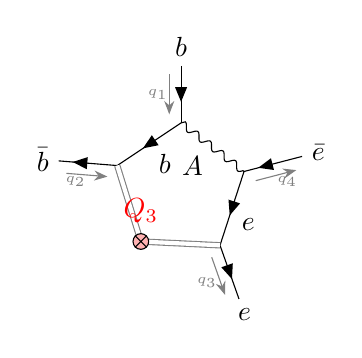
\begin{tikzpicture}
\tikzfeynmanset{}
\begin{feynman}
\diagram[small]{
   i1 [particle=$b$] -- [fermion, momentum'={[arrow style=gray, label distance=-1mm, arrow distance=1.5mm] {\tiny $q_{1}$}}] v1,
   i3 [particle=$\bar b$] -- [anti fermion, momentum'={[arrow style=gray, label distance=-1mm, arrow distance=1.5mm] {\tiny $q_{2}$}}] v2,
   v5 -- [fermion, momentum'={[arrow style=gray, label distance=-1mm, arrow distance=1.5mm] {\tiny $q_{3}$}}] o2 [particle=$e$], 
   v3 -- [anti fermion, momentum'={[arrow style=gray, label distance=-1mm, arrow distance=1.5mm] {\tiny $q_{4}$}}] o4 [particle=$\bar e$], 
   v1 -- [edge label=$b$, fermion] v2,
   v3 -- [edge label=$A$, boson] v1,
   v4 -- [double distance=1.5pt, gray] v2,
   v3 -- [edge label=$e$, fermion] v5,
   v5 -- [double distance=1.5pt, gray] v4,
};
\draw (v4) node [draw=black, shape=crossed circle, inner sep=2pt, fill=white!70!red, label={[red]$Q_3$}];
\end{feynman}
\end{tikzpicture}\\
\# $28$ \\
(symmetry: $+1$)
\end{center}
\end{minipage}
%
\end{document}
